\documentclass[a4paper,11pt]{article}
\pdfoutput=1 % if your are submitting a pdflatex (i.e.~if you have
             % images in pdf, png or jpg format)

\usepackage{jinstpub} % for details on the use of the package, please
\usepackage{caption}
\usepackage{subcaption}
\usepackage{float}
\usepackage{makecell}
\usepackage[T1]{fontenc}
\usepackage[utf8]{inputenc}
\usepackage{upgreek}

\usepackage[colorinlistoftodos,prependcaption,textsize=tiny]{todonotes} %todo note in margin
\newcommand{\answ}[1]{\todo[linecolor=blue,backgroundcolor=blue!25,bordercolor=blue]{#1}}

                     % see the JINST-author-manual


\title{Characterization of a beam tagging hodoscope for hadrontherapy monitoring}


%% %simple case: 2 authors, same institution
%% \author{A. Uthor}
%% \author{and A. Nother Author}
%% \affiliation{Institution,\\Address, Country}

% more complex case: 4 authors, 3 institutions, 2 footnotes
\author[a,1]{O. Allegrini,\note{Corresponding author.}}
\author[b]{J.-P. Cachemiche,}
\author[b]{C.P.C. Caplan,}
\author[a]{B. Carlus,}
\author[a]{X. Chen,}
\author[c]{S. Curtoni}
\author[c]{D. Dauvergne,}
\author[a]{R. Della Negra,}
\author[c]{M.-L. Gallin-Martel,}
\author[e]{J. H\'{e}rault,}
\author[d]{J.M. L\'{e}tang,}
\author[b]{C. Morel,}
\author[a]{\'{E}. Testa,}
\author[a]{and Y. Zoccarato.}

% The "\note" macro will give a warning: "Ignoring empty anchor..."
% you can safely ignore it.

\affiliation[a]{Univ. Lyon, Univ. Claude Bernard Lyon 1, CNRS/IN2P3, IP2I Lyon, F-69622, Villeurbanne, France.}
\affiliation[b]{Aix-Marseille Univ, CNRS/IN2P3, CPPM, Marseille, France.}
\affiliation[c]{Universit\'e Grenoble Alpes, CNRS, Grenoble INP, LPSC-IN2P3, UMR 5821, 38000 Grenoble, France.}
\affiliation[d]{Univ. Lyon, INSA-Lyon, Univ. Claude Bernard Lyon 1, UJM-Saint \'Etienne, CNRS, Inserm, CREATIS UMR 5220, U1206, F-69373, LYON, France.}
\affiliation[e]{Department of Radiation Oncology, Antoine-Lacassagne Cancer Center, Nice, France.}

% e-mail addresses: only for the forresponding author
\emailAdd{o.allegrini@ipnl.in2p3.fr}


\abstract{A beam tagging hodoscope prototype made of 500~$\upmu$m square silicon fibers arranged in two perpendicular planes and coupled to multi-anode photomultiplier have been studied using proton beams and various intensities. As a performance test, the beam tagging hodoscope successfully provided 2D image of proton beam. A detection efficiency $\geq$ 98\% was obtained with a logical OR condition between the two planes whereas close to 75\% were reached with a logical AND condition at low intensity (10$^{5}$~Hz). Moreover, the timing resolution was evaluated to 0.5~ns at low intensity, making this detector a viable technology for beam monitoring applications.}



\keywords{scintillating fibers, beam monitoring, hadrontherapy}


%\arxivnumber{1234.56789} % only if you have one

% \collaboration{\includegraphics[height=17mm]{example-image}\\[6pt]
%   XXX collaboration}
% or
%\collaboration[c]{on behalf of CLaRyS collaboration}


% if you write for a special issue this may be useful
%\proceeding{N$^{\text{th}}$ Workshop on X\\
  %when\\
  %where}

\usepackage{xcolor}
\colorlet{jmlcolor}{green!70!black}
\newcommand\jml[1]{\color{jmlcolor}JML: - #1 - \color{black}}

\begin{document}
\maketitle
\flushbottom

\section{Introduction}
\label{sec:intro}

Ion beam therapy is a rapidly expanding radiotherapy modality, with more than 250,000 patients being treated worldwide (https://www.ptcog.ch/index.php/patient-statistics). The main advantage of this technique lies in the dose conformity with the target volume resulting from the sharp Bragg peak observed in the dose profile at the end of the ion range. Moreover therapies with ions heavier than protons benefit from increased biological effect in the tumor region, hence enhancing the treatment effectiveness \cite{Braccini2010, Durante2016, Schardt2010, Paganetti2013, Jakel2008}. However, this therapy technique faces uncertainties concerning the Bragg peak position mainly due to X-ray imaging modalities, anatomical changes of the patient during the treatment, organ motion and approximations used in dose calculation \cite{Paganetti2012}. 
As a consequence, the most widespread treatment planning techniques are performed with several beam incidences accomodating treatment robustness at the expense of higher doses in healthy tissues. Moreover, additional safety margins are applied around the tumor volume to ensure the full irradiation of  tumor cells \cite{Durante2016, Knopf2013}.

In this context, clinically applicable methods and instruments are under development to control \textit{in vivo} ion ranges and dose profiles with millimeter accuracy by means of secondary radiation detection. Such systems exploit the production of $\beta$+ emitters during nuclear reactions undergone by a fraction of incident ions. At present, offline PET/CT range verification is performed in some hadrontherapy centers to provide ion-range control after the treatments. The exploitation of these particles currently continues with the development and clinical tests of in-beam PET scanners for online ion beam monitoring \cite{Shao2014, Ferrero2018}.
Nuclear reactions also lead to the emission of prompt gammas (PG) that can be considered for ion-range verification \cite{Krimmer2018}. Several PG modalities are under development worldwide and a few of them make use of time-of-flight (TOF) measurement either to derive indirect information on ion-ranges (Prompt Gamma Timing, PGT \cite{Golnik2014, Marcatili2020}) or to reduce neutron-induced background \cite{Fontana2020, Dal_Bello_2020, Aldawood2017}. Most of beam monitoring systems currently implemented in clinical facilities, based on ionization chambers \cite{Stelzer2002}, are not designed to monitor the Bragg peak position. These new devices will thus contribute to the reinforcement of the quality assurance check.

TOF measurement requires a time reference corresponding to the arrival of incident ions or ion bunches, depending on the beam time structure. The use of the accelerator radio-frequency (RF) as time reference would have the advantage of simplicity, when there is a perfect periodicity and short ion bunches (cyclotron accelerators). However the precise correlation between the RF phase and the ion/bunch arrival can be only obtained in mono-energetic beam conditions. 
Indeed the use of degraders to change beam energies in cyclotrons introduces a time dispersion and shifts of bunches. Moreover small variations of the cyclotron’s magnetic field also slightly affect the orbital frequency of the ion trajectories. Hence a small phase shift per turn can appear between ion trajectory and RF signal resulting in a measurable mismatch which varies in time \cite{Werner2019}. 
Several devices under development based on scintillating fibers provide particles tracking with integration \cite{Leverington2018} or particle-per-particle \cite{Horikawa2004, Achenbach2008, Braccini2012} acquisition mode for various fields of application, including proton radiography \cite{Presti2013} and ion-range verification during hadrontherapy \cite{PAPA2016}. Recently, the performance of a time-tracker for a prompt-gamma spectroscopy system allowing for a background TOF rejection with a sub-nanosecond time resolution has been demonstrated \cite{Martins2020}. One of the scintillating fibers hodoscope currenlty developed is the one of the ClaRyS collaboration, which is dedicated to be coupled with a PG imaging system (collimated- or Compton-camera). The expected detection efficiency of the beam tagging hodoscope is over 90\% for coincidence events in the X and Y planes whereas a time resolution below 2~ns has to be reached. Furthermore, the count rate of the device has to be compatible with a clinical beam intensity.

This paper presents reports of tests of this hodoscope performed at ion beams. At first, performance tests were performed at GANIL with 95~MeV/u carbon ions to measure the detection efficiency as well as the variation of the scintillating fibers response as a function of the beam fluence. Then, the setting method and the results of the in-beam characterization of the beam tagging hodoscope, performed during two measurements campaigns, at Centre Antoine Lacassagne (CAL), in Nice, are presented. Multiplicity, detection efficiency and time resolution were assessed. 

\section{Material and methods}
\subsection{The beam tagging hodoscope}

The beam tagging hodoscope of the CLaRyS collimated and Compton cameras is dedicated to provide a spatiotemporal tagging of ion (or ion bunches) passages for a beam intensity up to 10$^{8}$~Hz.
The final version of the beam tagging hodoscope is composed  of 1~mm$^{2}$ squared section polystyrene scintillating fibers BCF-12 manufactured by Saint-Gobain. These fibers are cladded with a thin layer of acrylic, the thickness of which corresponds to 4\% of the fiber size. Their emission peak is located at 345~nm with a time decay of 3.2~ns \cite{SaintGobain2017}.
The beam tagging hodoscope is constituted of two perpendicular planes of fibers. Each plane contains 128 fibers, which gives an active area of 128$\times$128~mm$^{2}$. A black tape covers the sensitive area to provide a shielding against external light. Fibers are readout on both side by 8 Hamamatsu multi-anode photomultipliers (PM) H8500C. The number of read-out channels is then 512. Connections with fibers are made in such a way that a same fiber is read-out by two neighboring channels of a PM and two adjacent fibers are handled with different PMs. This configuration will allow to optimize the detector efficiency and to improve the time resolution.  Figure~\ref{fig:hodoscope} shows the prototype.

\begin{figure}[htb]
\centering
\includegraphics[width=0.4\textwidth]{figures/Beam_Tagging_Hodoscope.png}
\caption{\small{\textit{Large version of the beam tagging hodoscope.}}}
\label{fig:hodoscope}
\end{figure}

Each PM is linked to a front-end (FE) card via 64-channel connector where signals are processed by two application specific integrated circuits (ASIC) (32 channels per ASIC). The ASICs provide a trigger based on a logical OR operated on all channels. Generating the trigger requires a few ns and is subject to exceeding a current threshold. For that, the signal amplitude has to be greater than the fixed threshold for a duration over about 1.5~ns, in order not to be lost. Thus, two categories of signals can be collected in the FE board: the enable pulses, on the one hand, are events whose intensity exceeds the threshold during a time sufficient to be processed. On the other hand, the short pulses correspond to undesired events for which a PM signal cross the threshold over a too short time period for the ASIC to handle the signal. PM channel gains and ASIC thresholds can be tuned to improve the data collection and improve the signal-to-background ratio (cf \ref{Settings}).

A time-to-digital converter (TDC) based on a 160~MHz clock is implemented in ASICs, allowing to tag the time of the detected events. An analog to digital converter (ADC) is used to measure the charge received by a single channel. When the charge exceeds the fixed threshold, a trigger is generated. The collected data in the two ASICs are sent to the FPGA after being processed by the ADC. Three main functions are allocated to the FPGA: the data-stream processing, the slow-control and the data transmission. Finally, the data are sent from FPGA to acquisition system via a 3~Gbit$\cdot$s$^{-1}$ optical fiber thanks to the transmission module of the FPGA. \cite{deng2013, Chen2017, Chen2019}.

For this study, a smaller hodoscope with 32 fibers per plane has been developed in order to use a single acquisition board to collect all the data of the two planes.


\subsection{General principle of the experimental setups}

Figure \ref{fig:Picture_Setup_hodo} illustrates the setup used for the in-beam tests.
The hodoscope, placed on its custom mechanical support, is surrounded on each side by two plastic scintillators (PS), in such a way that any projectile triggering a coincidence in the two PS impacts also the tested detector: this can be made with reduced size PS, or sufficiently small-area beam spot to avoid triggering PS coincidence without impinging the beam tagging hodoscope. These two PS are aligned with the beam and located about 5 cm upstream and downstream of the hodoscope (cf figure \ref{fig:Picture_Setup_hodo}). The signals of these detectors are read out by PM which are connected to a Nuclear Instrumentation Module (NIM) where the analog data are converted in logic signals via a preset threshold. This configuration allowed to generate double (two PS) and triple coincidences (two PS AND the beam tagging hodoscope: either the OR or the AND of the two planes). Then the ratio of triple coincidence to double coincidence is a direct measure of the tested detector efficiency in the area encompassing the detectors and the beam spot. This configuration allows the monitoring of the beam intensity up to a value close to {10}$^{5}$~ions$\cdot$s$^{-1}$.

\begin{figure}[htb]
\centering
\includegraphics[width=0.5\textwidth]{figures/Experimental_setup_hodoscope_March_August_2019_marked.pdf}
\caption{\small{\textit{Experimental setup with the beam tagging hodoscope placed between the two PS.}}}
\label{fig:Picture_Setup_hodo}
\end{figure}


\subsection{GANIL experiments}

The radiation damage assessment was performed with the small hodoscope, connected to a single PM biased at 800~V. Discrete NIM electronics were used for discrimination, charge integration and timing (Time to Amplitude Converter). The discriminator threshold was set at 30~mV, which corresponds to about 1/6th of the maximum of the amplitude distribution. The effect of radiation damage was estimated by repeating efficiency measurement (see above), after a given number of irradiation periods at high intensity.

\subsection{Centre Antoine Lacassage (CAL) experiments}
\label{In-beam_tests}

A third PS has been installed out of the beam irradiation field in order to monitor the beam intensity, by the measurement of secondary emissions, when the two PS in the beam are saturated. This detector was calibrated at low beam intensity with the in-beam detectors. Futhermore, a calibration between the PS and the intensity measured in the cyclotron stripper. After being sent to the coincidence module, the signal of the two scintillators, upstream and downstream of the hodoscope, is handled in a discriminator. The output signal of this last module is used as a stand-alone trigger signal in the FE card. 

The fiber signal in coincidence with the trigger signal, in a 11~ns acceptance time window, is sent to the AMC40 card through a 3~Gbit$\cdot$s$^{-1}$ signal-channel optical link with a specific protocol and then to the PC with DAQ software for data processing via 1~Gbit$\cdot$s$^{-1}$ ethernet link. Both optical and Ethernet links also transmit slow control package, which is used for calibration by a PC implemented a LabVIEW-based program (cf figure \ref{fig:Scheme_Setup_hodo}). 

At the same time, the three single independent signals and the coincidence module output signal are recovered by the LabView-based program to visualize the counting rate and estimate the beam intensity in real time.
Finally, during the beam test an additional PC was used to tune the coincidence windows via a JTAG link.

\begin{figure}[htb]
\centering
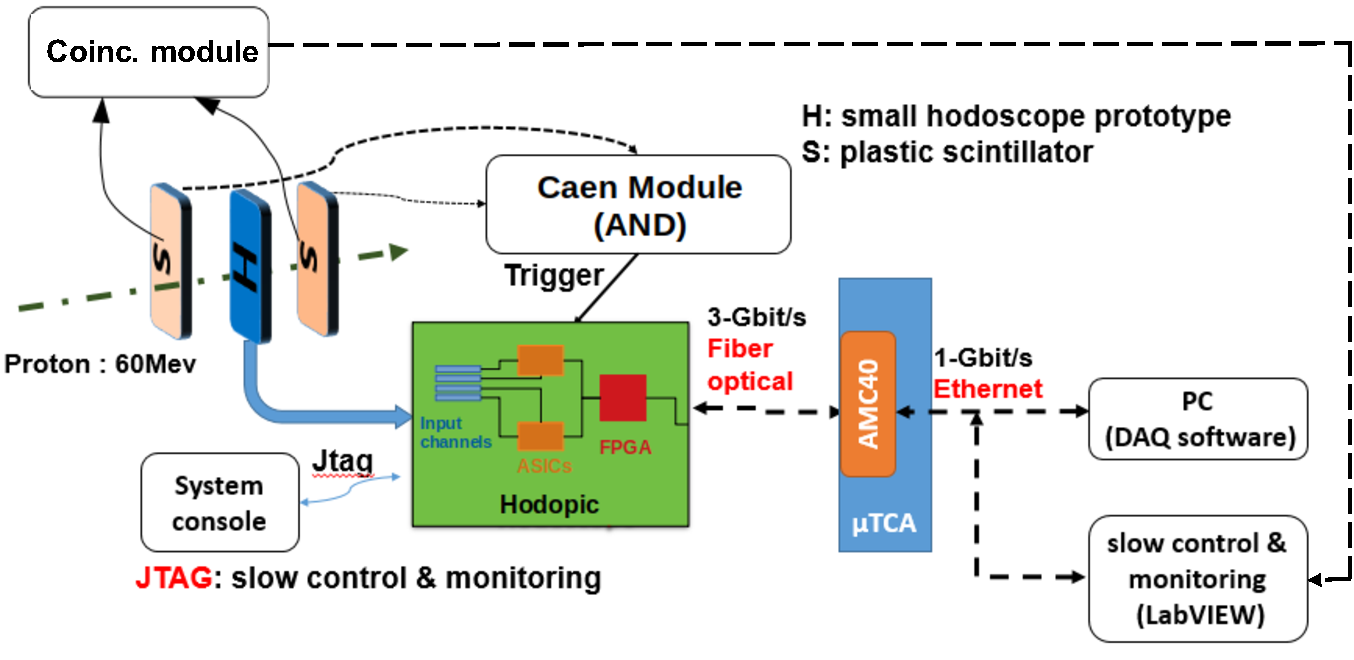
\includegraphics[width=0.8\textwidth]{figures/Scheme_Setup_Nice_08_2019.pdf}
\caption{\small{\textit{Scheme of the data acquisition chain of the experimental setup.}}}
\label{fig:Scheme_Setup_hodo}
\end{figure}

The MEDICYC low energy treatment line of the CAL is intended for the treatment of ocular tumors. The research area of this beam line is located a few meters upstream of the treatment room. The maximum beam energy is 64.5~MeV and the high frequency of the accelerator is of 24.85~MHz so that the beam consists of proton bunches arriving every 40.24~ns. Throughout the rest of the paper, beam intensities are expressed in Hz because the mean number of protons per bunch is always below 1 for the range of intensities used during these experiments. The counting rates recorded in the PS are approximated to Hz unit.
The performance of the hodoscope is mainly assessed in terms of detection efficiency and spatial resolution. Multiplicity and profiles are also considered in this characterization study.

\subsection{Criteria and settings}
\label{Settings}

A condition to set the PM channel gains and the ASIC thresholds is to assess the cross-talk between neighboring pixels. For this, the PMs have been scanned with a blue LED and results showed a retrieved cross-talk more important than provider specifications but always below 3\% for the tested anodes which is sufficiently low to be easily rectified by an adapted threshold setting \cite{FontanaPhD}.

As regards the setting method to configure the ASIC thresholds and channel gains, a logic periodic signal with a given frequency has been sent to each input channel, one by one. Enable and short pulses are stored as a function of the threshold for all gains ranging from 0.25 to 3.75 by step of 0.25. The obtained curves, named S-Curve, have a typical shape as shown in figure \ref{fig:S_Curve}. The enable curve presents a range of thresholds for which signals are collected followed by a sharp fall-off (point B in figure~\ref{fig:S_Curve}). In this same region, a rising edge can be observed in the short-pulse curve. Another region with an high rate of short pulse signal located at low threshold values can be noticed (below point A in figure~\ref{fig:S_Curve}). These signals are related to background events. The method used to determine a set of gains and threshold is based on three main steps:
\begin{itemize}
\item A first scan of the input channels consists in determining the noisiest channel for the minimal gain (0.25), i.e.~the channel for which the noise’s threshold (point A in figure \ref{fig:S_Curve}) is the highest. Thus a reference range of suitable thresholds is determined between the points A and B.
\item Suitable threshold values in the reference interval for the other channels are recorded.
\item The selection of the “optimal” threshold corresponds to the value for which the ratio between enable and short pulses is maximum for the highest number of channels. The gain of channels not meeting this criterion is enhanced step by step until the optimum is reached.
\end{itemize}
%The following beam test was dedicated to assess the correction of an artifact in the firmware impacting the time resolution (cf \ref{Time_resolution}).

\begin{figure}[htb]
\centering
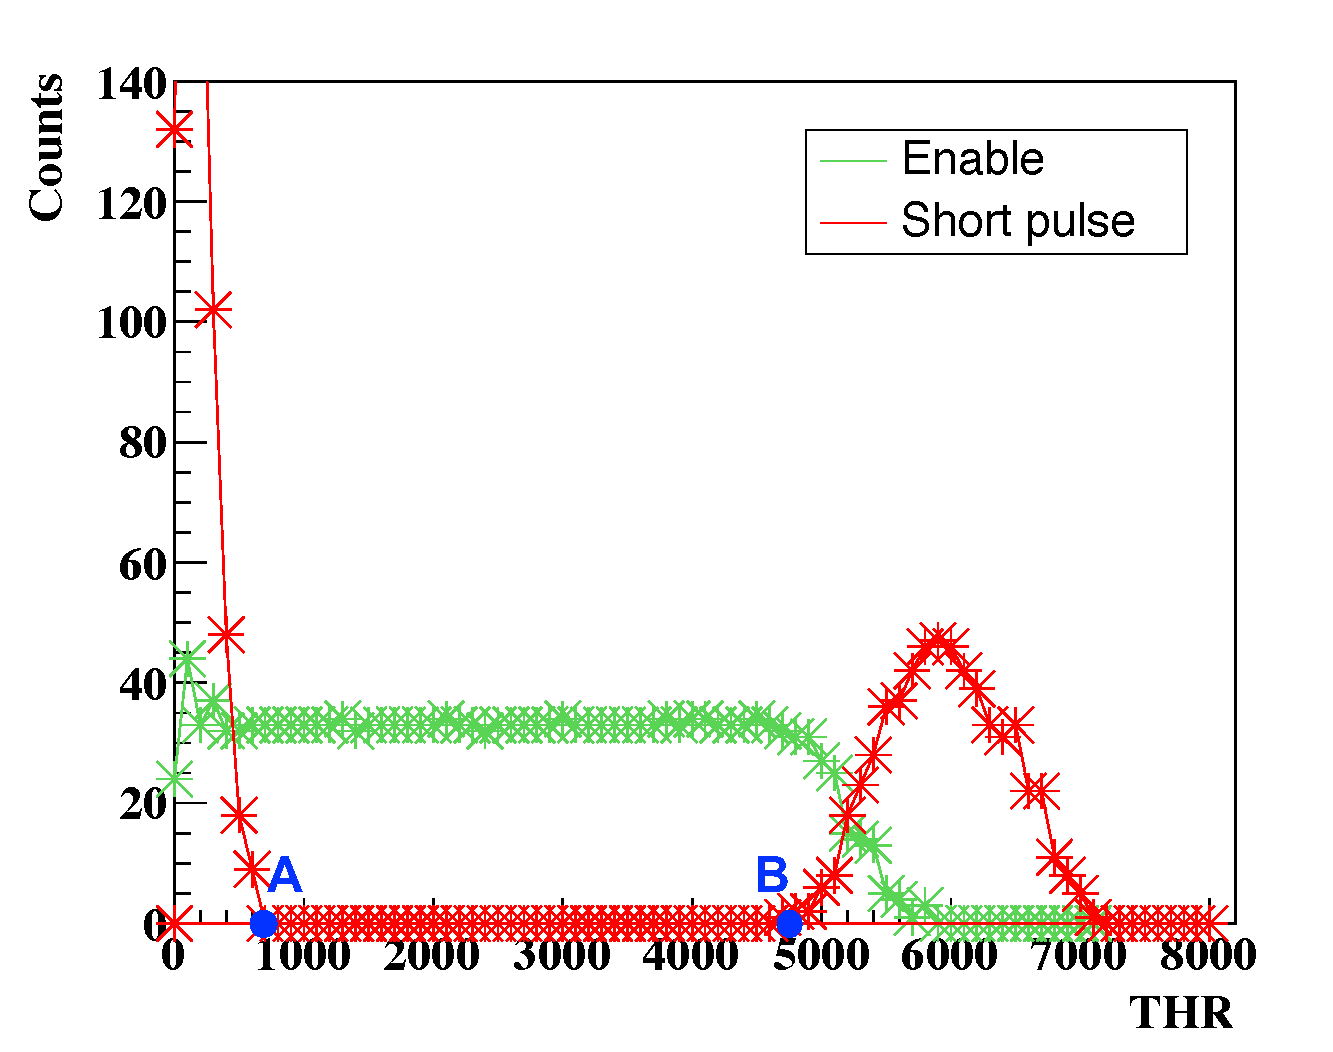
\includegraphics[width=0.5\textwidth]{figures/S_Curve_Thr_suitable_rangeAB.pdf}
\caption{\small{\textit{Number of "enable" and "short pulse" events as a function of the threshold (THR) for a given channel. The range between points A and B corresponds to a suitable threshold range for this channel.}}}
\label{fig:S_Curve}
\end{figure}

\section{Results}
\subsection{Experiment with carbon ions at GANIL}
A total detection efficiency of 94\% was obtained with a single plane, while the fraction of events with multiplicity > 1 represented 24\%, mainly due to cross talk between adjacent channels of the multi-anode PM.
From SRIM estimation \cite{Ziegler2010}, the energy deposit in a 1~mm thick plastic fiber is 26~MeV. The results for the integrated charge per projectile, and the measured efficiency, are reported in table \ref{tab:GANIL}. A significant decrease of the efficiency was measured after 2.2$\times$10$^{12}$~ions$\cdot$cm$^{-2}$, but it was almost recovered by lowering the threshold. 
Close to 90\% detection efficiency was kept after 3.6$\times$10$^{12}$ ions$\cdot$cm$^{-2}$.
Concerning the irradiation damages, it should be noted that after few days, a partial restoration of the response at laboratory test benches has been observed, but it was not possible to repeat the detection efficiency measurement with carbon ions. 
The time resolution was measured between one fiber output and the cyclotron high frequency signal, and assessed to 550~ps RMS. 
\begin{table}[htb]
\caption{\small{\textit{Evolution of the hodoscope response with carbon ion fluence. The detection efficiency is measured on a single fiber plane with a multi-anode PM H8500 and a power supply of 800~V. A threshold of 30~mV corresponds to 4.5~pC measured on QDC.}}}
\centering
\begin{tabular}{|c|c|c|c|c|c|}
\hline
Fluence (cm$^{-2}$)& 0 & (7.2$\pm$1.2)$\times$10$^{11}$ & (2.2$\pm$0.4)$\times$10$^{12}$ & (2.2$\pm$0.4)$\times$10$^{12}$ & (3.6$\pm$0.7)$\times$10$^{12}$\\
\hline
\makecell{Discriminator\\threshold (mV)} & 30 & 30 & 30 & 15 & 15\\
\hline
\makecell{Mean QDC\\value (pC)} & 35 & 34 & 27 & 21 & 21\\
\hline
Efficiency (\%) & 94 & 94 & 63 & 92 & 86\\
\hline
\end{tabular}
\label{tab:GANIL}
\end{table}

\subsection{Experiments with protons at CAL}
\subsubsection{Profiles and Multiplicities}
\label{Profiles_And_Multiplies}

The multiplicity (M) is defined as the number of involved fibers per plane when a trigger is generated.
Figure \ref{fig:Multiplicity} presents the multiplicity of both planes for three beam intensities: 17~kHz, $\sim$1.3~MHz and $\sim$20~MHz. The mean number of protons per bunch is 6.8$\times$10$^{-4}$, 5.2$\times$10$^{-2}$ and 8.0$\times$10$^{-1}$ respectively. The Poisson distribution of the number of proton per bunch for bunches having at least 1 proton is superimposed for each beam intensity since it corresponds to the expected multiplicity if we neglect the multiple proton arrivals in a single fiber. The probability for X$ = 0$ is not considered since bunches without proton do not trigger. 

Distributions of multiplicities at 17~kHz and $\sim$1.3~MHz are consistent with the Poisson distributions. Indeed, the ratio of events for which M$\leq$1 is close to 0.9 and 0.8 for X and Y planes respectively. However, at 20~MHz, this ratio decreases to 0.63 in X and 0.54 in Y plane and the events with M$\geq$1 is the majority. In general, M>1 in Y plane is higher 10$\pm$3.4\% than that of the X plane.
\begin{figure}[htb]
\centering
    \begin{subfigure}{0.32\textwidth} \centering 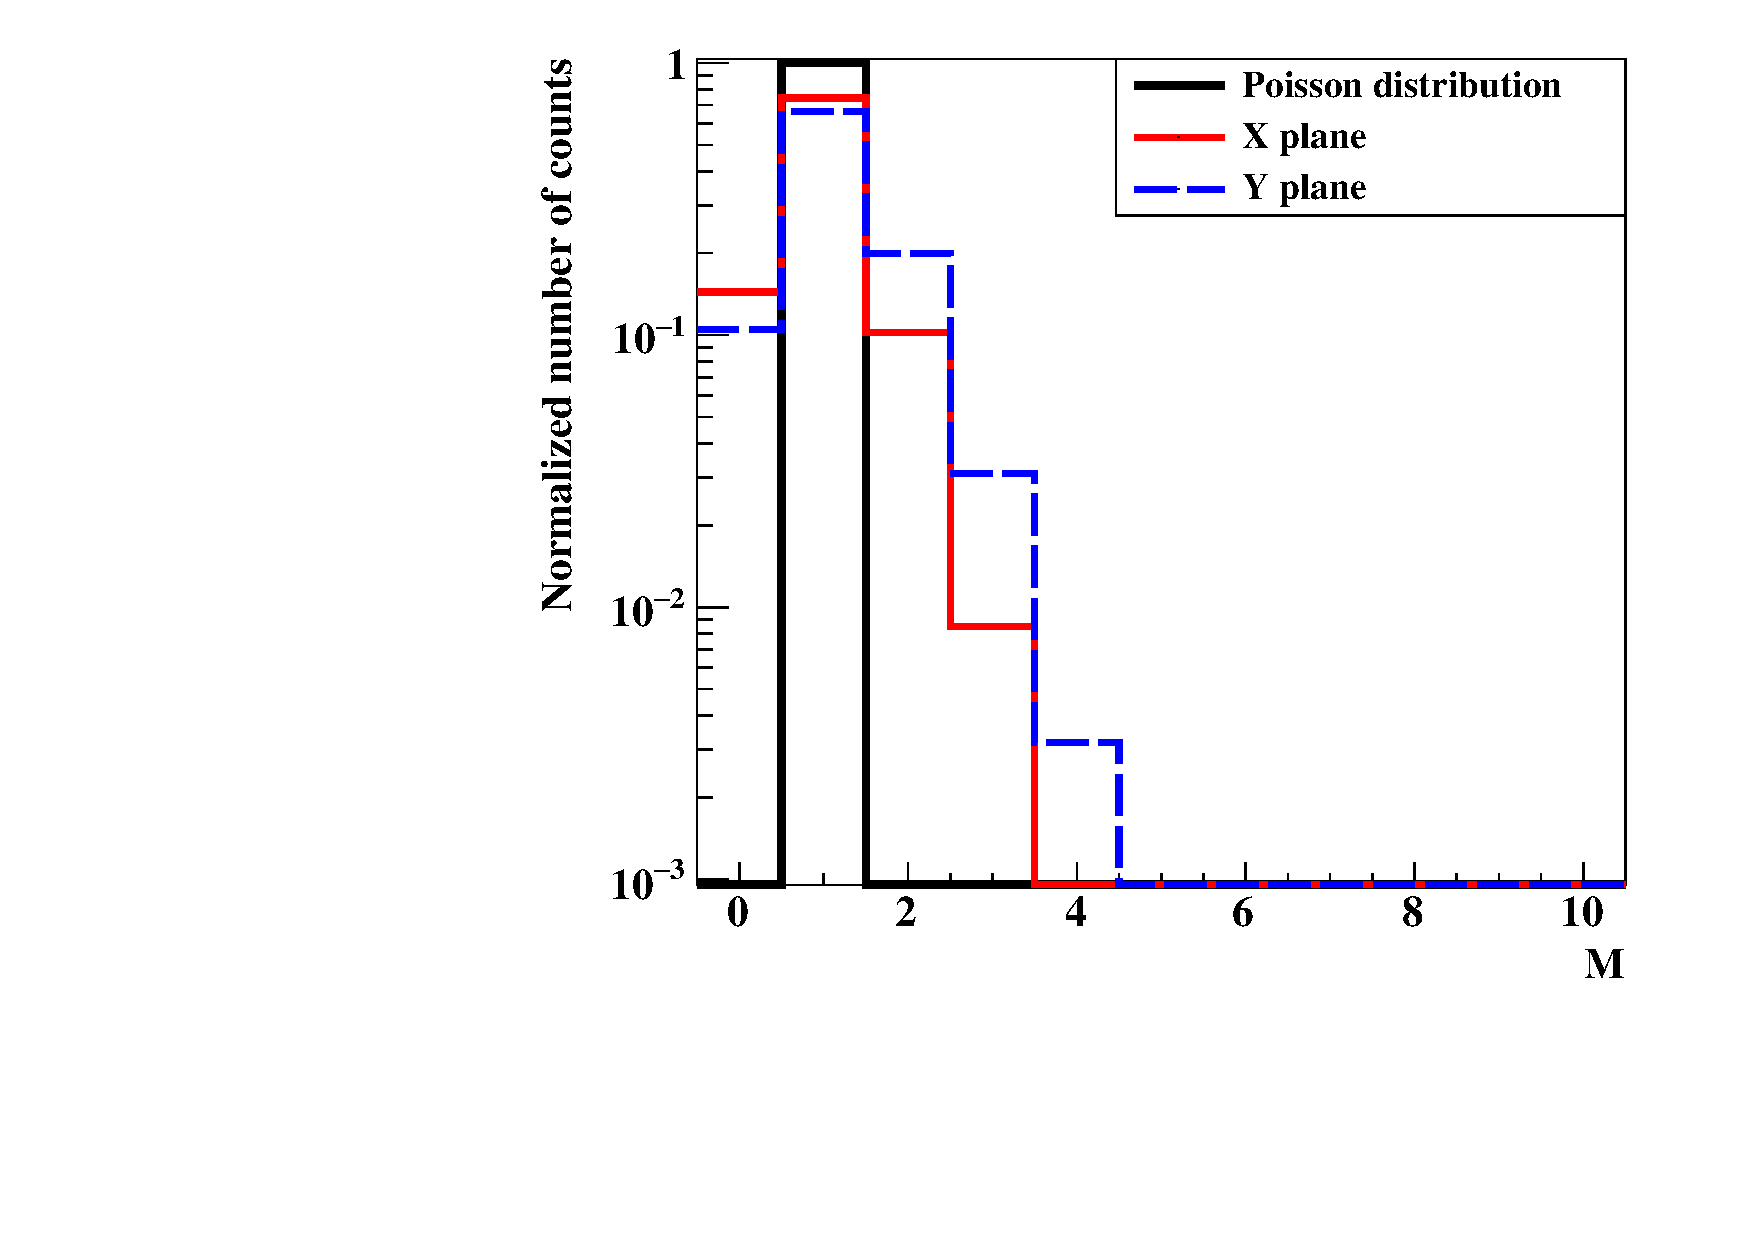
\includegraphics[width=\textwidth]{figures/Involved_fibers_17kHz_without_X=0.pdf} \caption{} \label{fig:Fibers_17kHz}
    \end{subfigure}
    \begin{subfigure}{0.32\textwidth} \centering 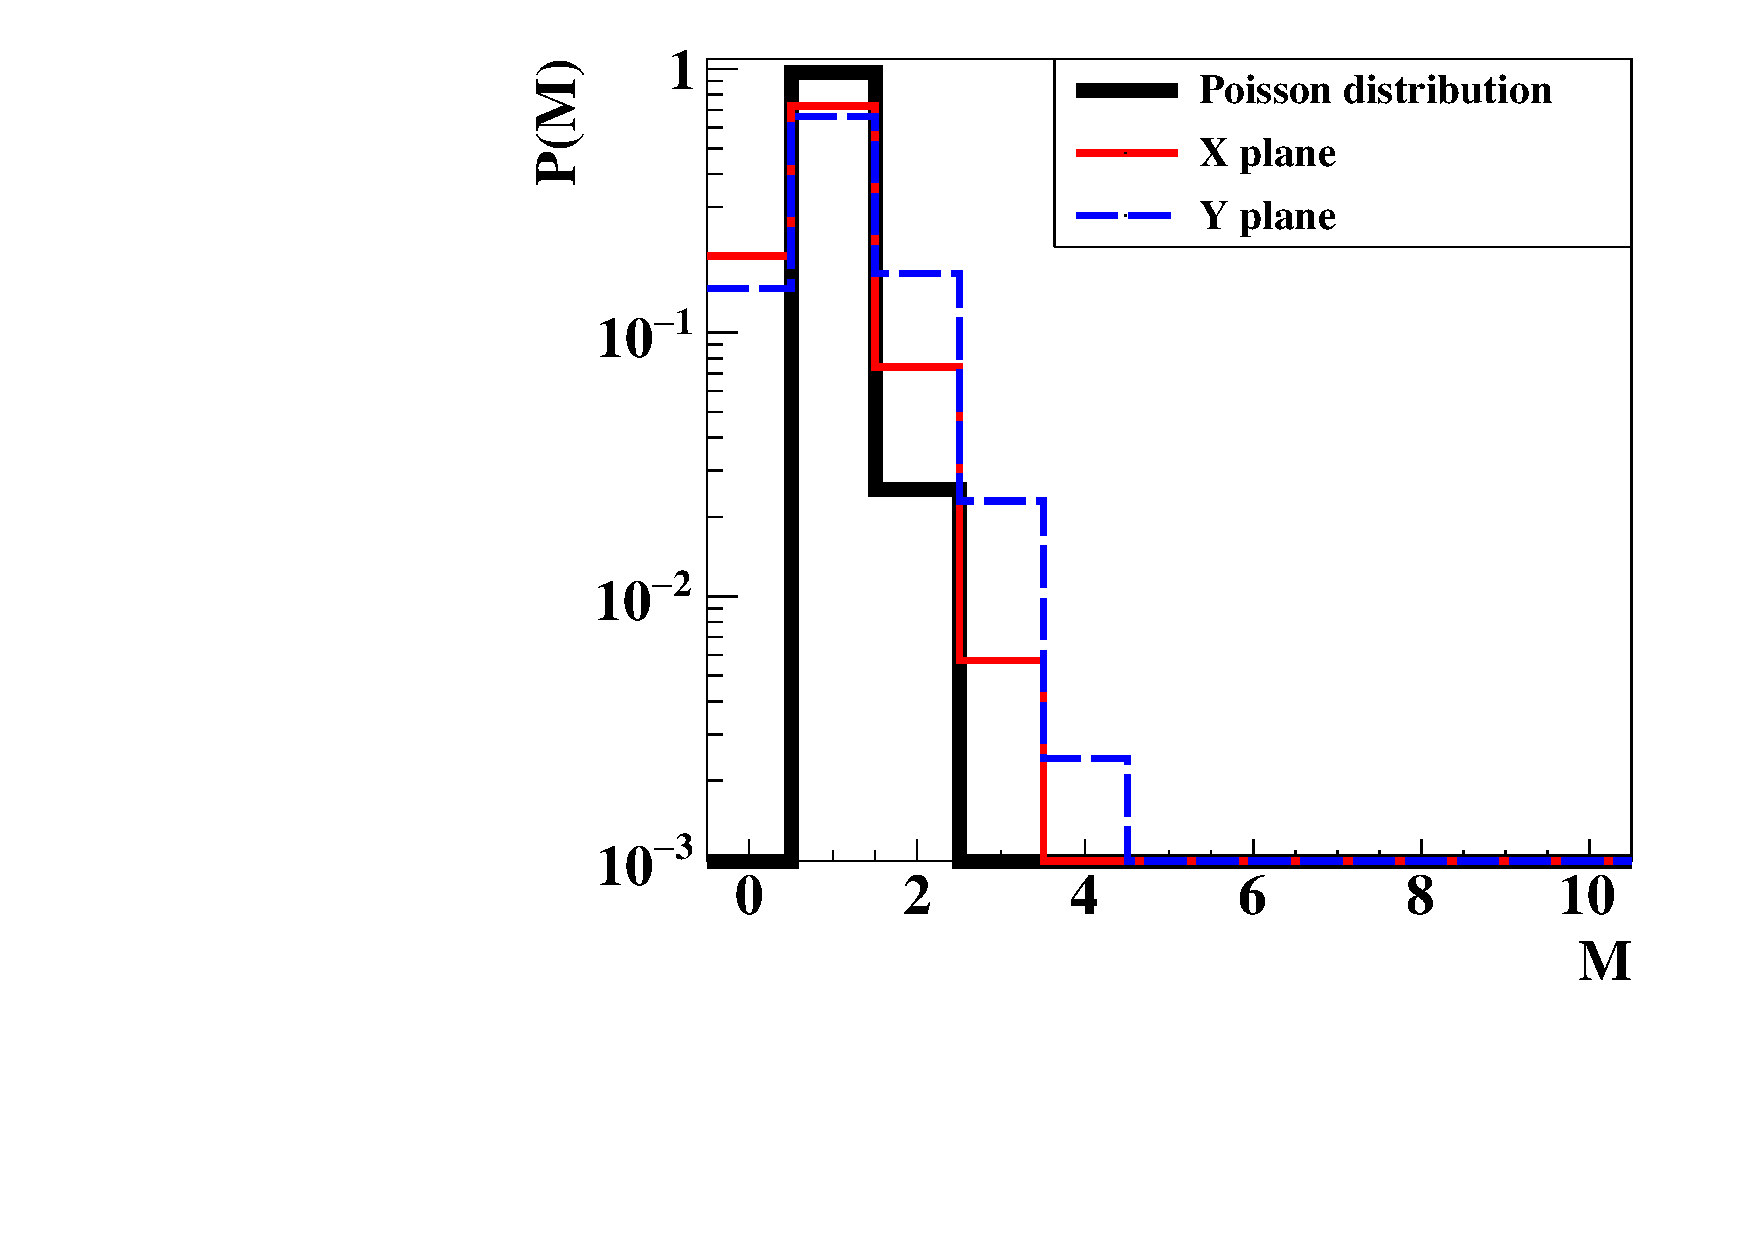
\includegraphics[width=\textwidth]{figures/Involved_fibers_1MHz_without_X=0.pdf} \caption{} \label{fig:Fibers_1MHz}
    \end{subfigure}
    \begin{subfigure}{0.32\textwidth} \centering 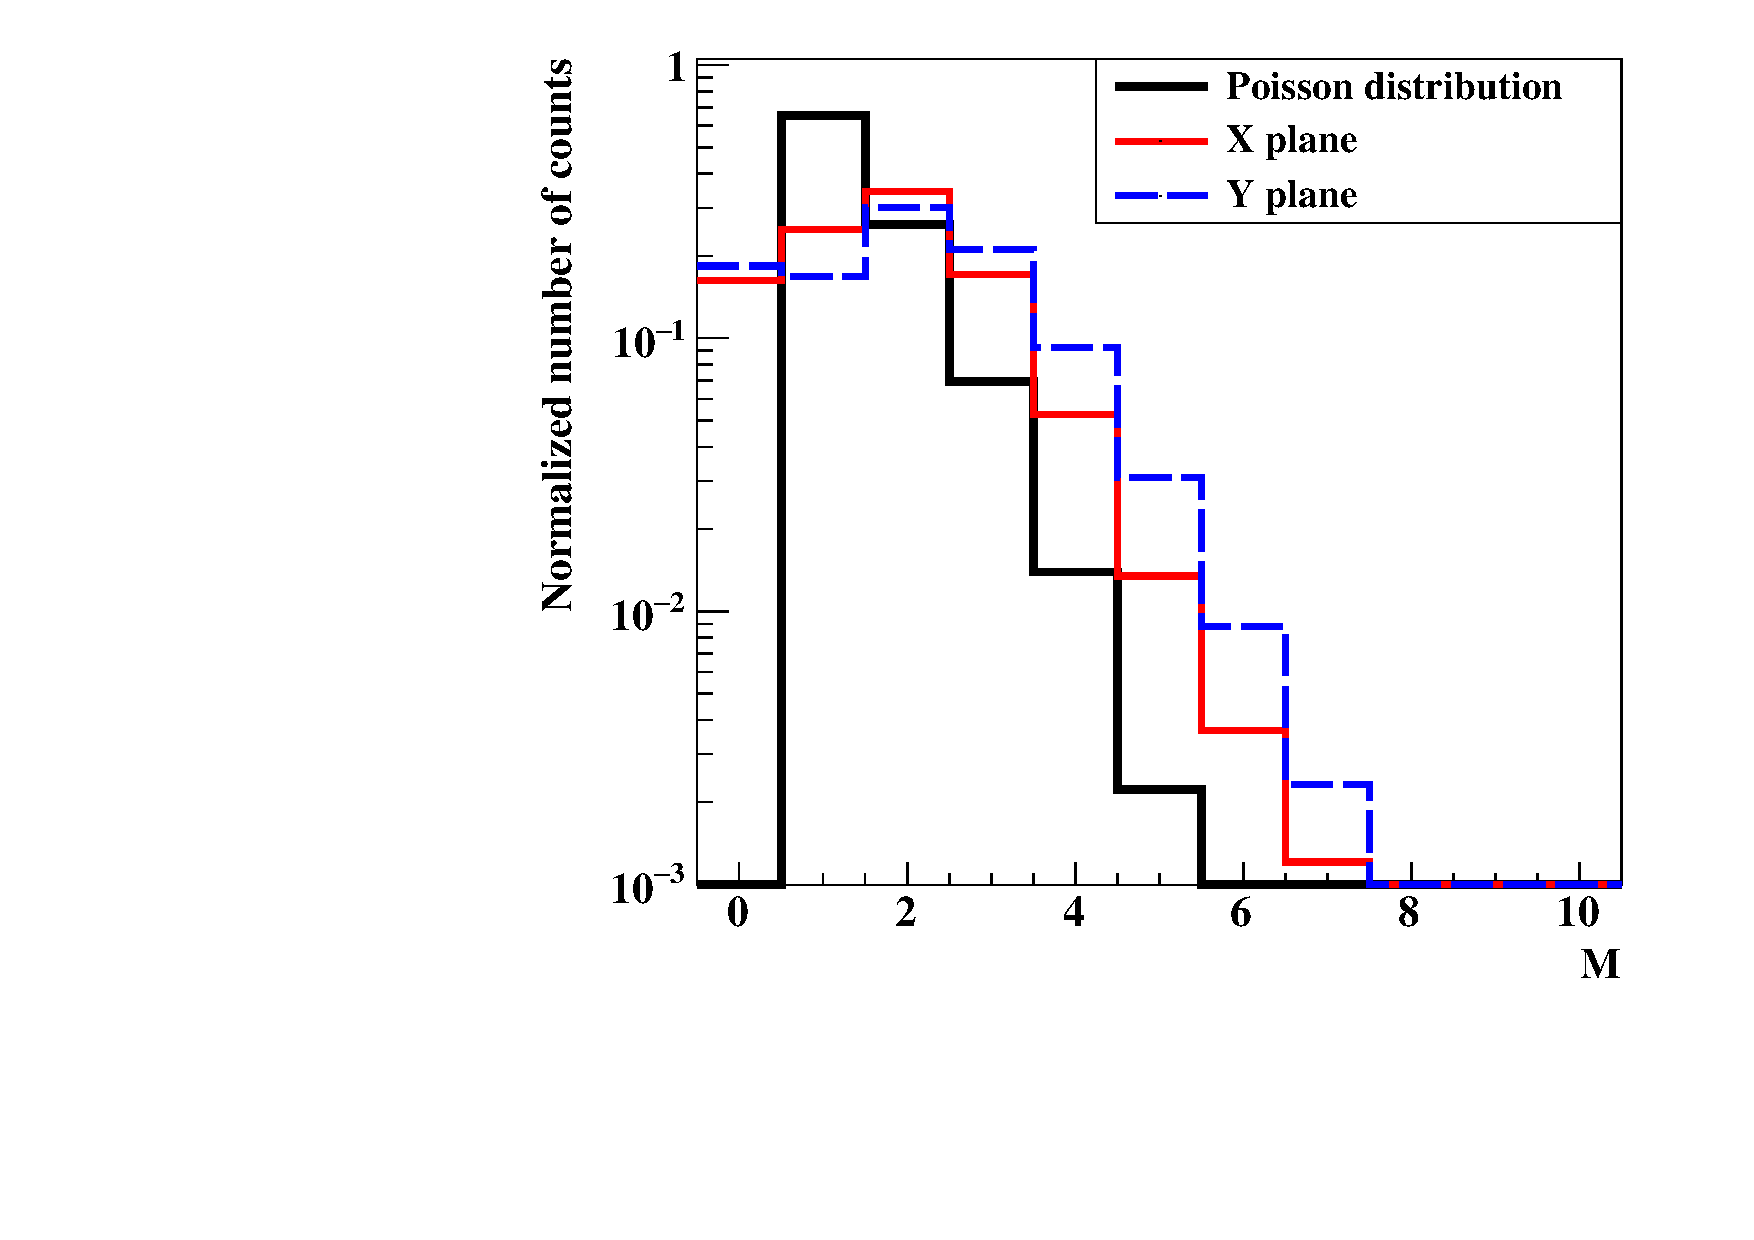
\includegraphics[width=\textwidth]{figures/Involved_fibers_20MHz_without_X=0.pdf} \caption{} \label{fig:Fibers_20MHz}
    \end{subfigure}
\caption{\small{\textit{Distribution of multiplicity for beam intensity of (a) 17 kHz, (b) $\sim$1.3 MHz and (c) $\sim$20 MHz.}}}
\label{fig:Multiplicity}
\end{figure}

The monitoring software reconstructs two-dimensional maps for each acquisitions. Figure~\ref{fig:2D_Maps} represents maps obtained for acquisition at 17~kHz and $\sim$20~MHz. The method of the reconstruction uses the  average position in X and Y for events with M > 1. Although the shape of the beam varies between the two intensities, the center of the beam is clearly defined. This modification could be due to the change of the focusing lens of the beam when the intensity increases. Moreover, a variability of the fiber response can be noticed in both planes.

\begin{figure}[htb]
\centering
    \begin{subfigure}{0.45\textwidth} \centering 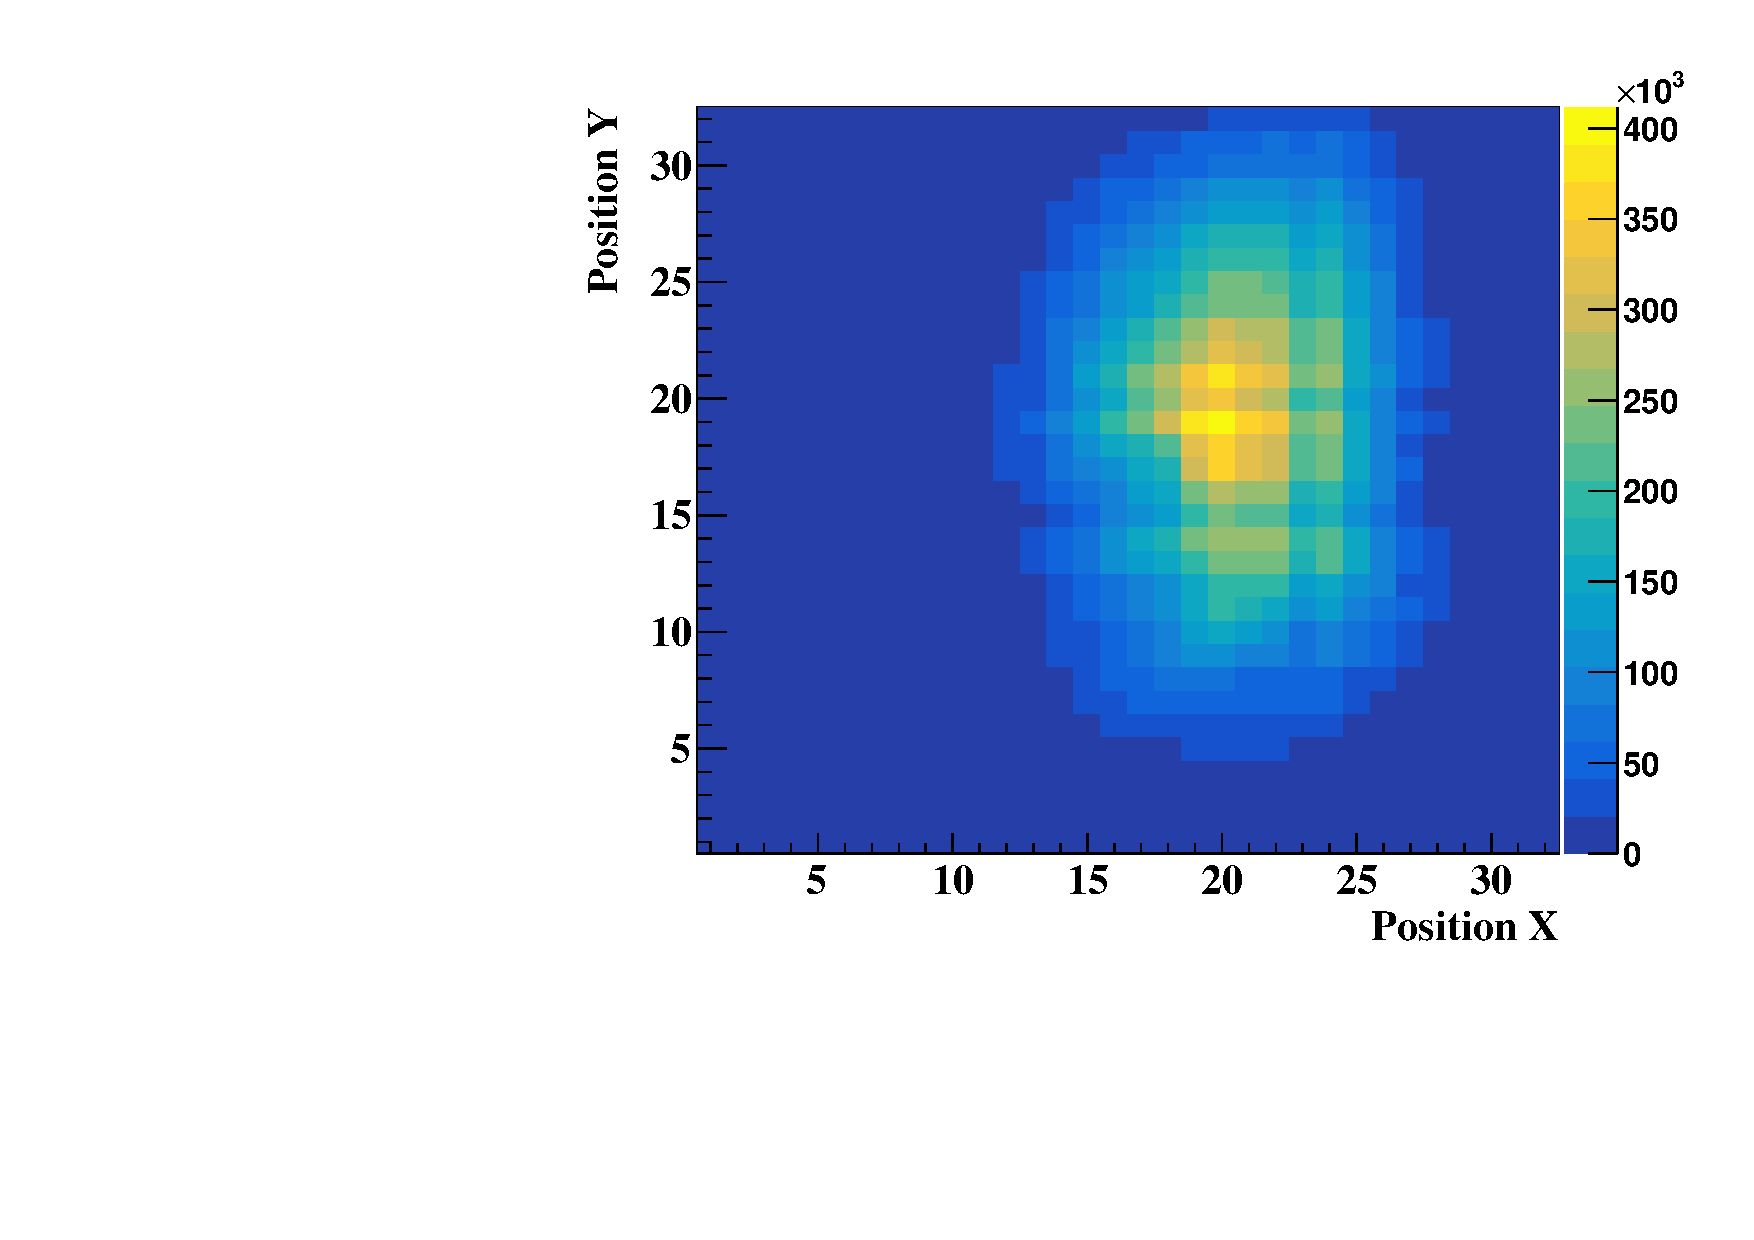
\includegraphics[width=\textwidth]{figures/2D_Map_1MHz.pdf} \caption{} \label{fig:2D_1MHz}
    \end{subfigure}
    ~
%\newline
%\centering
    \begin{subfigure}{0.45\textwidth} \centering 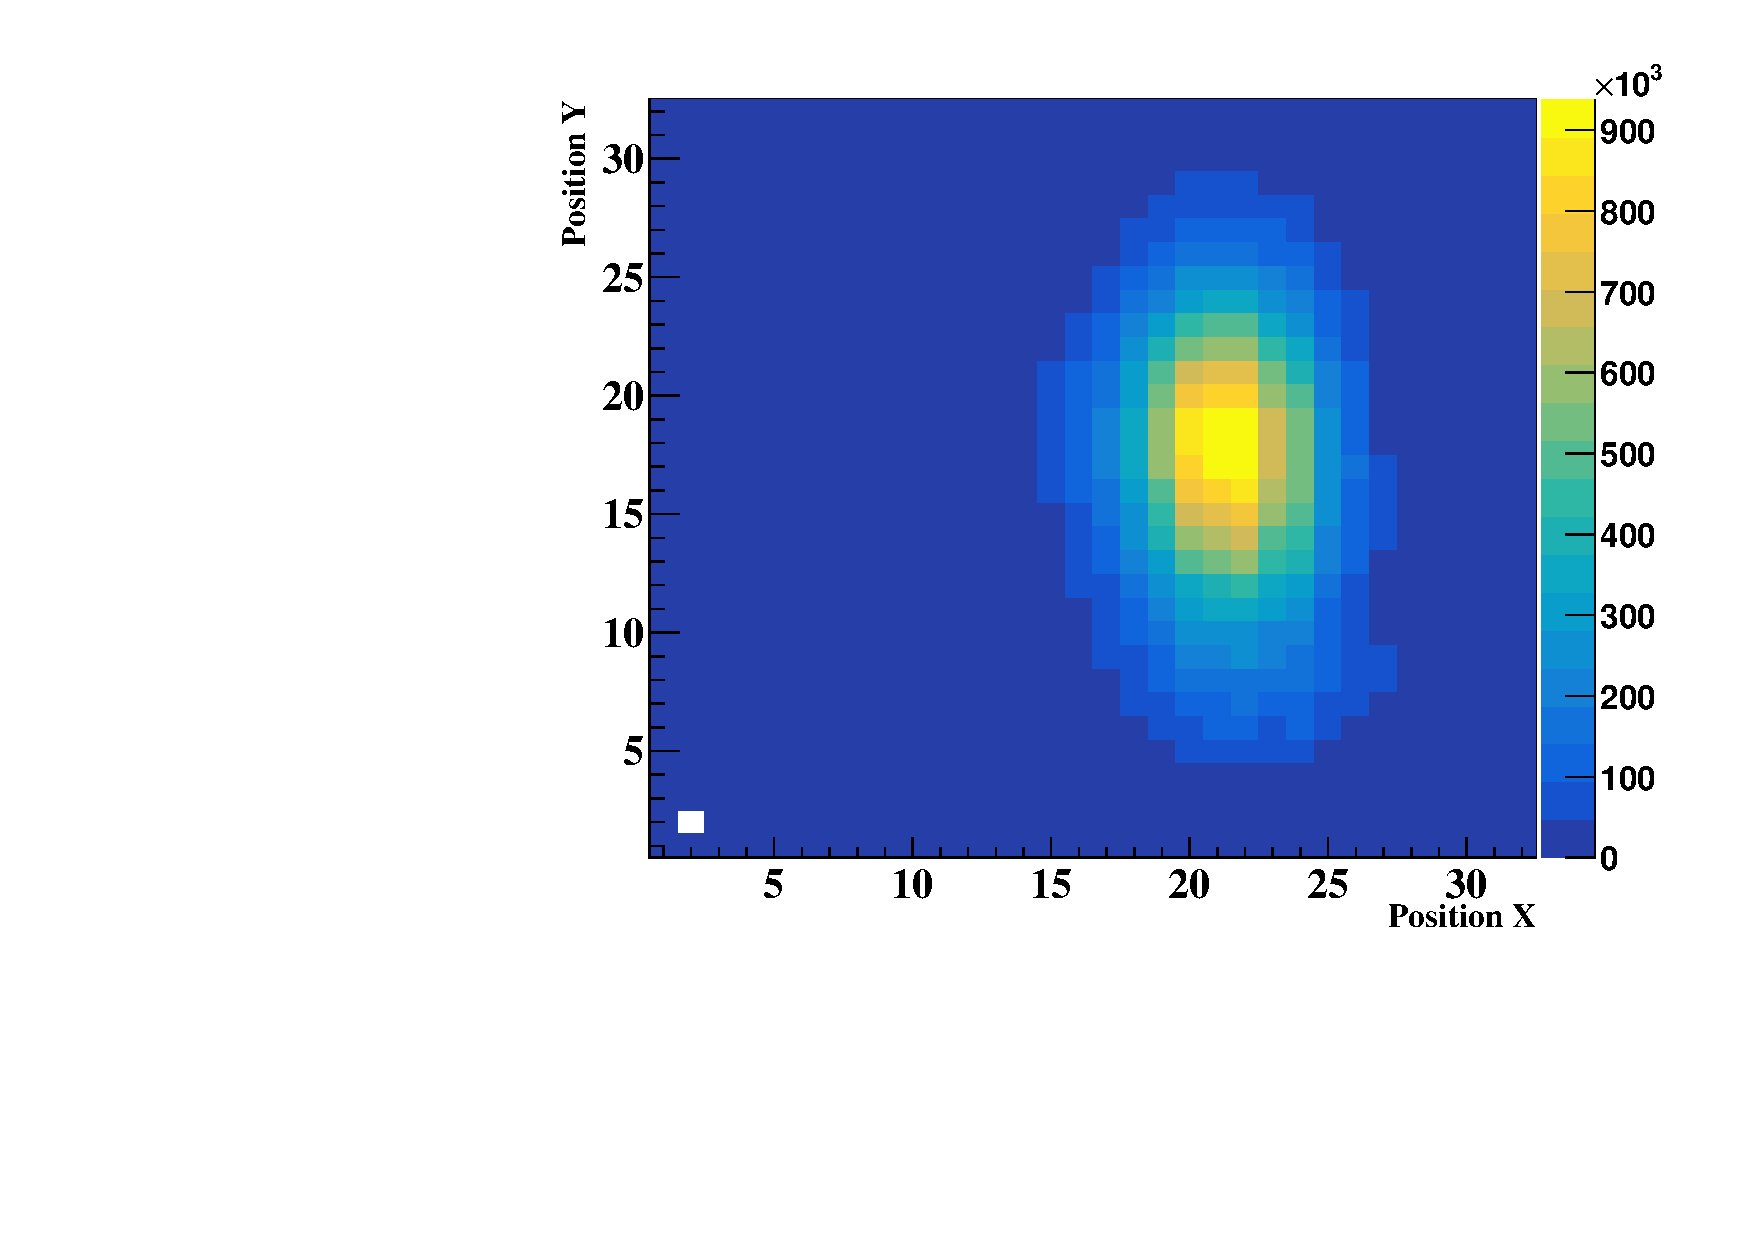
\includegraphics[width=\textwidth]{figures/2D_Map_20MHz.pdf} \caption{} \label{fig:2D_20MHz}
    \end{subfigure}
\caption{\small{\textit{2D map reconstruted from data collection for a beam intensity of (a) $\sim$1.3 MHz and (b) $\sim$20 MHz.}}}
\label{fig:2D_Maps}
\end{figure}

The variability of the fiber response has been assessed from the 1D profiles of both planes. Figure \ref{fig:1D_Profiles} represents the X and Y profiles obtained with two events selection methods for the irradiation with a beam intensity of $\sim$1.3~MHz. The blue curves correspond to the method used  for the 2D map reconstruction (average position of events with M>1). The red curve, meanwhile, represents only the events with M=1. The good overlap between the curves in both planes confirms the method used for the 2D map reconstruction is adapted. However, for intensities $\geq$ $\sim$20~MHz, the overlap of the two curves is strongly degraded.

\begin{figure}[htb]
\centering
    \begin{subfigure}{0.47\textwidth} \centering 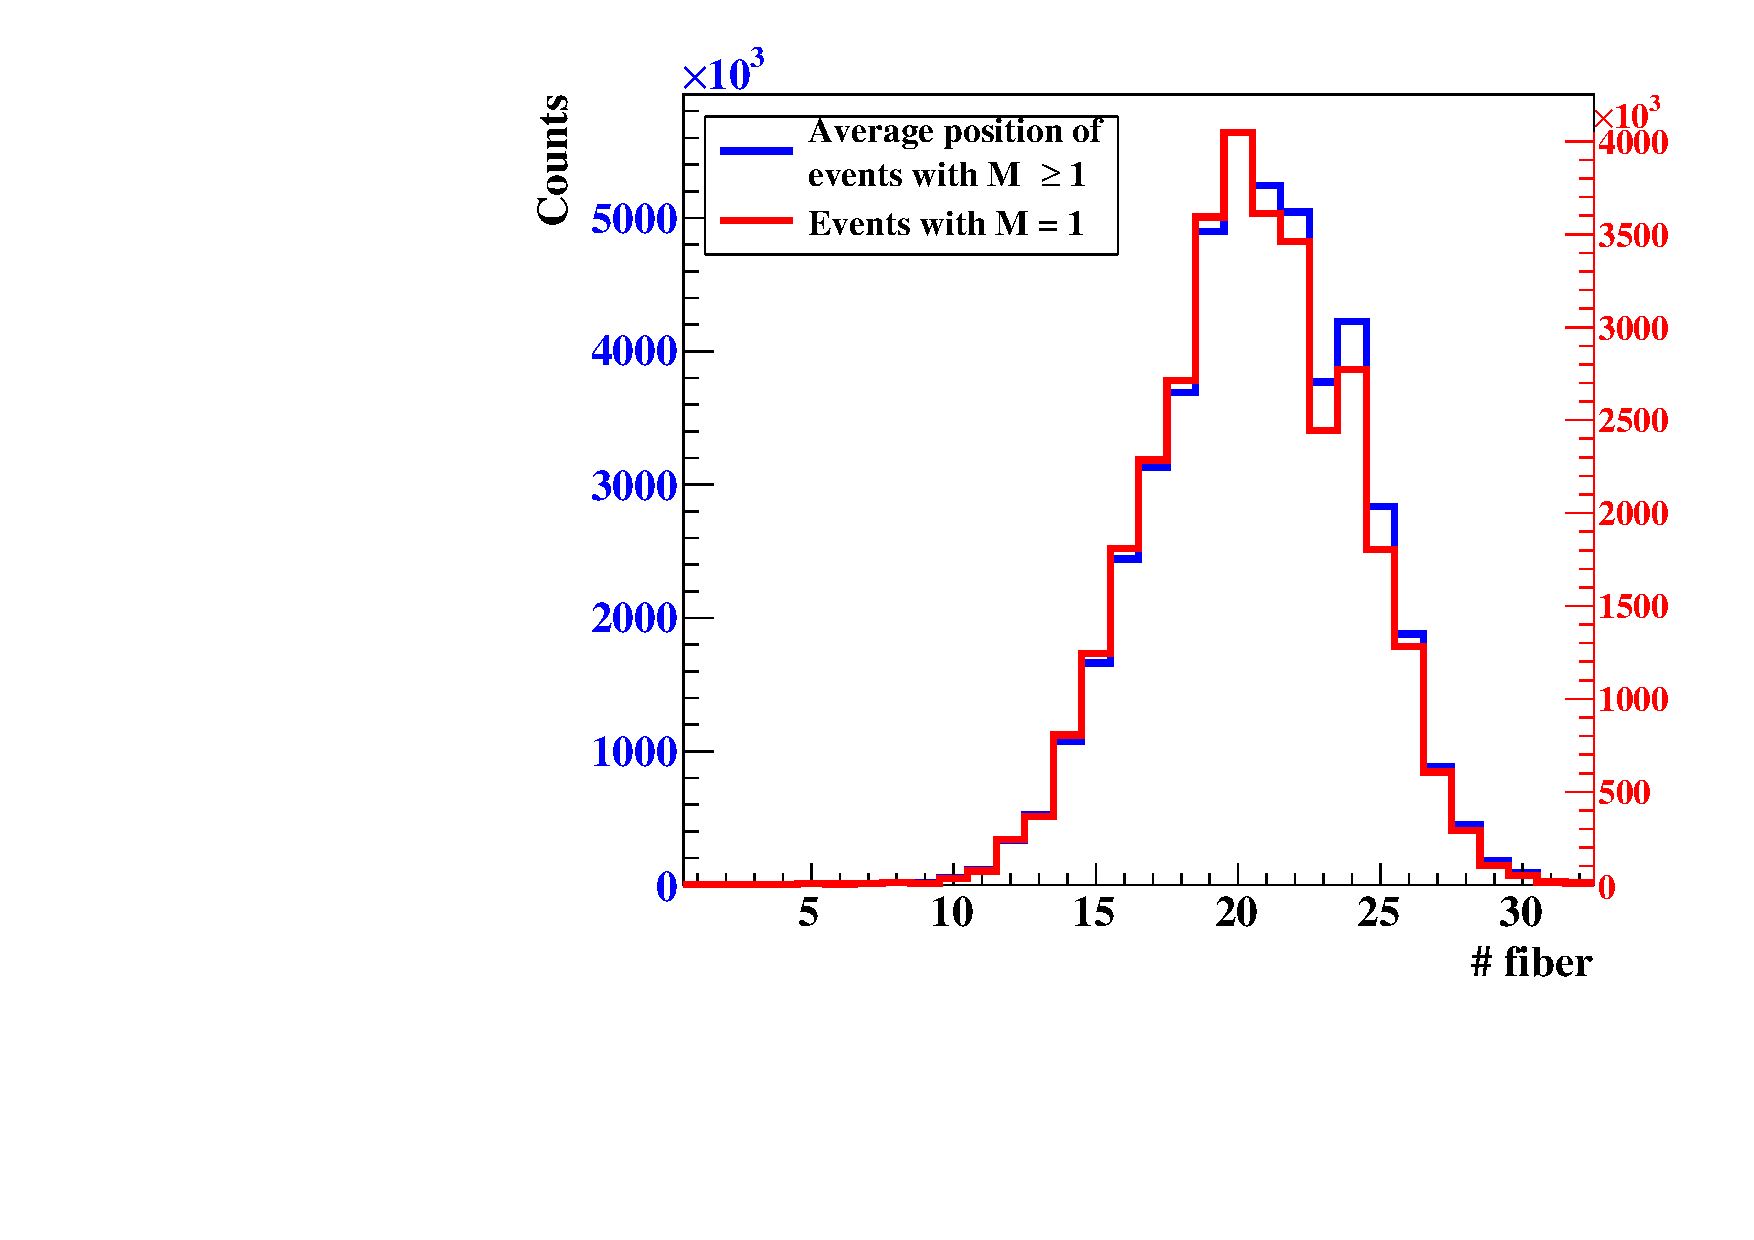
\includegraphics[width=\textwidth]{figures/Plane_X_1MHz.pdf} \caption{} \label{fig:Plane_X_1MHz}
    \end{subfigure}
    ~
    \begin{subfigure}{0.47\textwidth} \centering 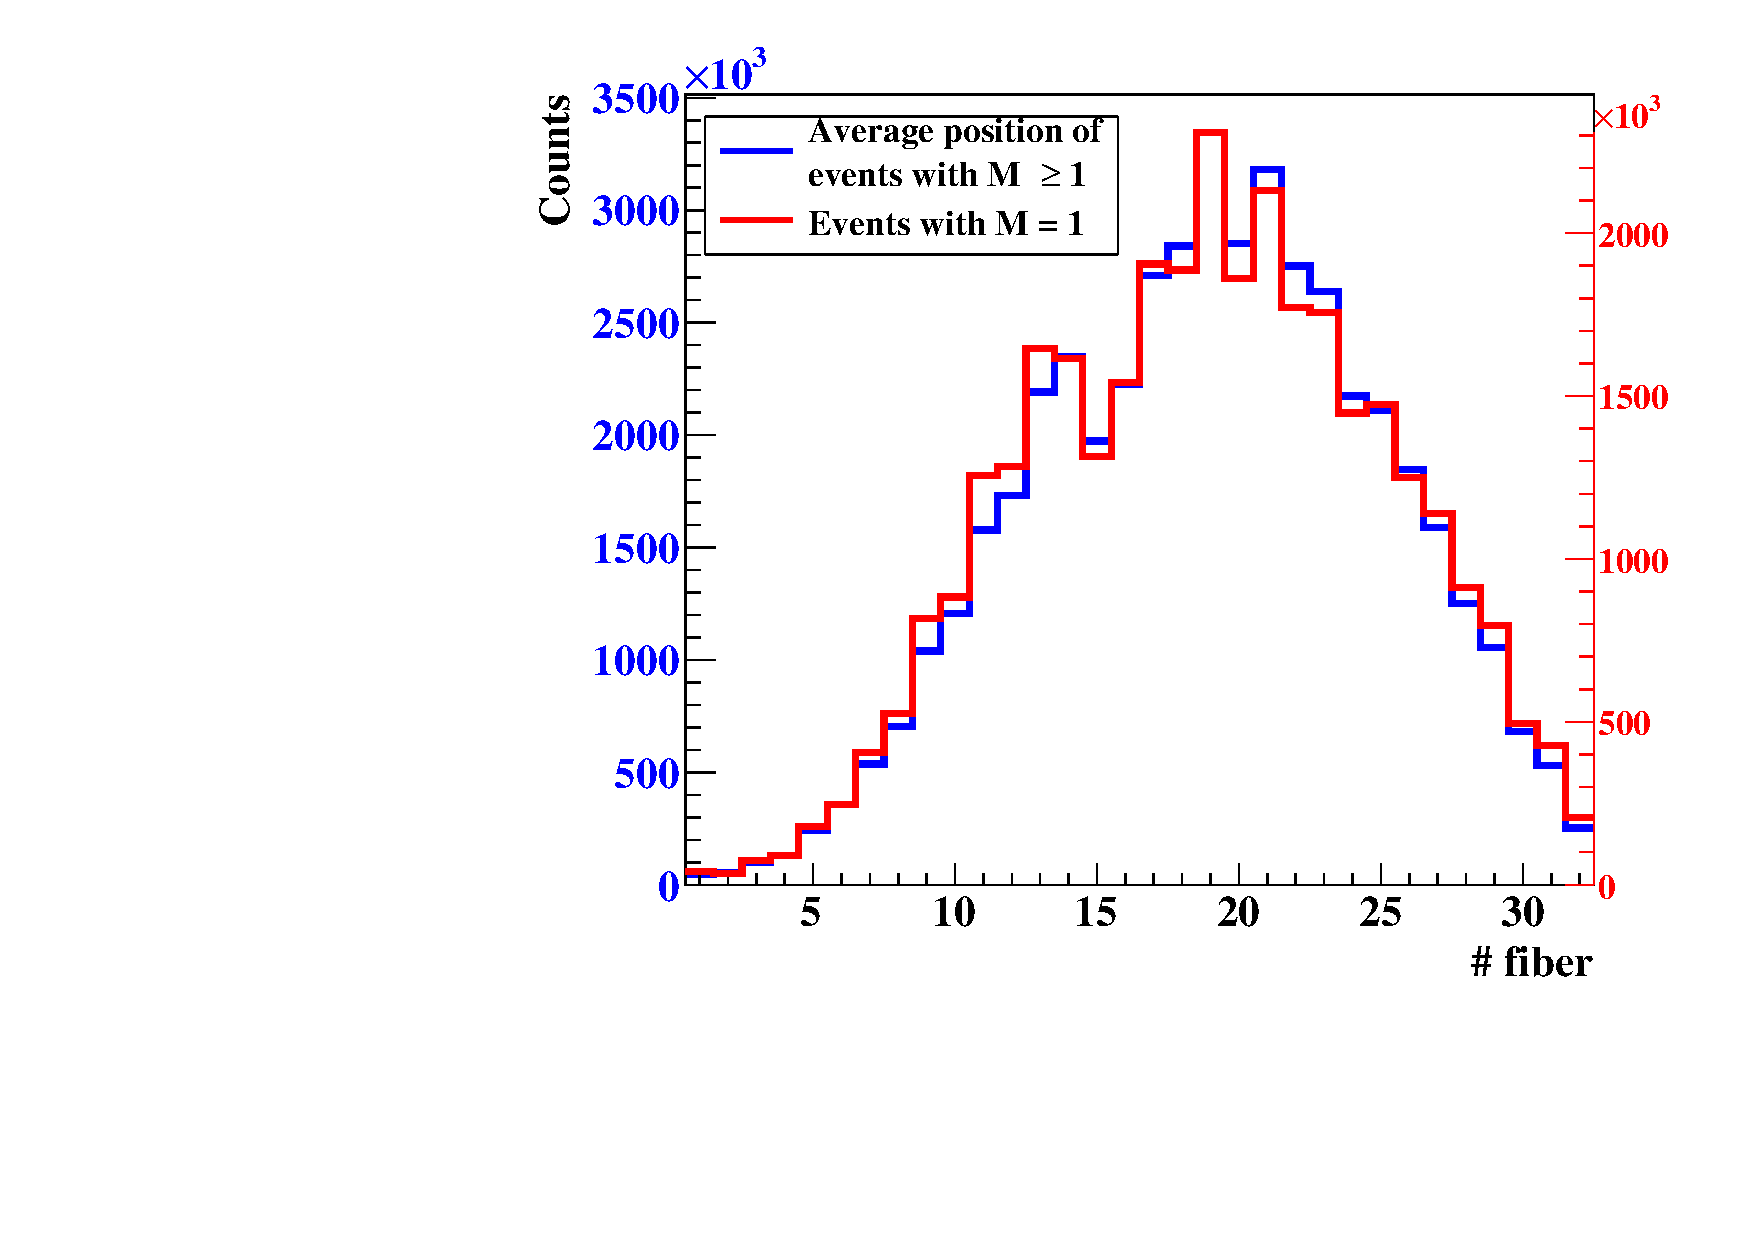
\includegraphics[width=\textwidth]{figures/Plane_Y_1MHz.pdf} \caption{} \label{fig:Plane_Y_1MHz}
    \end{subfigure}
\caption{\small{\textit{1D profiles of (a) X and (b) Y fiber planes with multiplicity M=1 and M$\geq$1 for a beam intensity of $\sim${1.3}~MHz.}}}
\label{fig:1D_Profiles}
\end{figure}

This phenomenon can be explained by the low number of events with M=1 in regard to the electronic noise which strongly increases for this range of intensity. The X and Y profiles highlight again the under-response of some fibers in the two planes. The latter has been evaluated by applying a linear interpolation on the fibers 23 in X and 15, 16 and 20 in Y plane to take it into account in the determination of the detection efficiency. The correction factor applied depends on the beam intensity because, as explained previously, the shape and the position of the beam in the hodoscope change with the intensity. The detection efficiency is corrected by a factor varying from 0.75\% to 4\% (resp.~2.7\% to 4\%) in the X (resp.~Y) plane.


\subsubsection{Detection efficiency}

Figure \ref{fig:DE} represents the detection efficiency of X and Y planes separately and with logical OR and AND conditions on the data of both planes, corrected for the under-response of fibers (cf \ref{Profiles_And_Multiplies}), for various intensities from 2~kHz to $\sim$20~MHz.
The detection efficiency in X plane keeps almost constant between 82.4\% and 84.8\% while in Y plane, it slightly varies from 88.3\% to 90.5\% for intensities under $\sim$6~MHz. A significant fall-off is of the detection efficiency is observed at $\sim$20~MHz (80.7\%). The logical OR condition on both planes allowed to obtain an high detection efficiency rate varying from 98\% to 99.2\%.
Concerning the coincidence detection efficiency with logical AND between X and Y fibers, the estimation is between 70.9\% and 74.5\% for intensity range from 2~kHz to $\sim$6~MHz. A noticeable decrease can be observed for intensity $\sim$20~MHz for which the detection efficiency is 65.4\%.

\begin{figure}[htb]
\centering
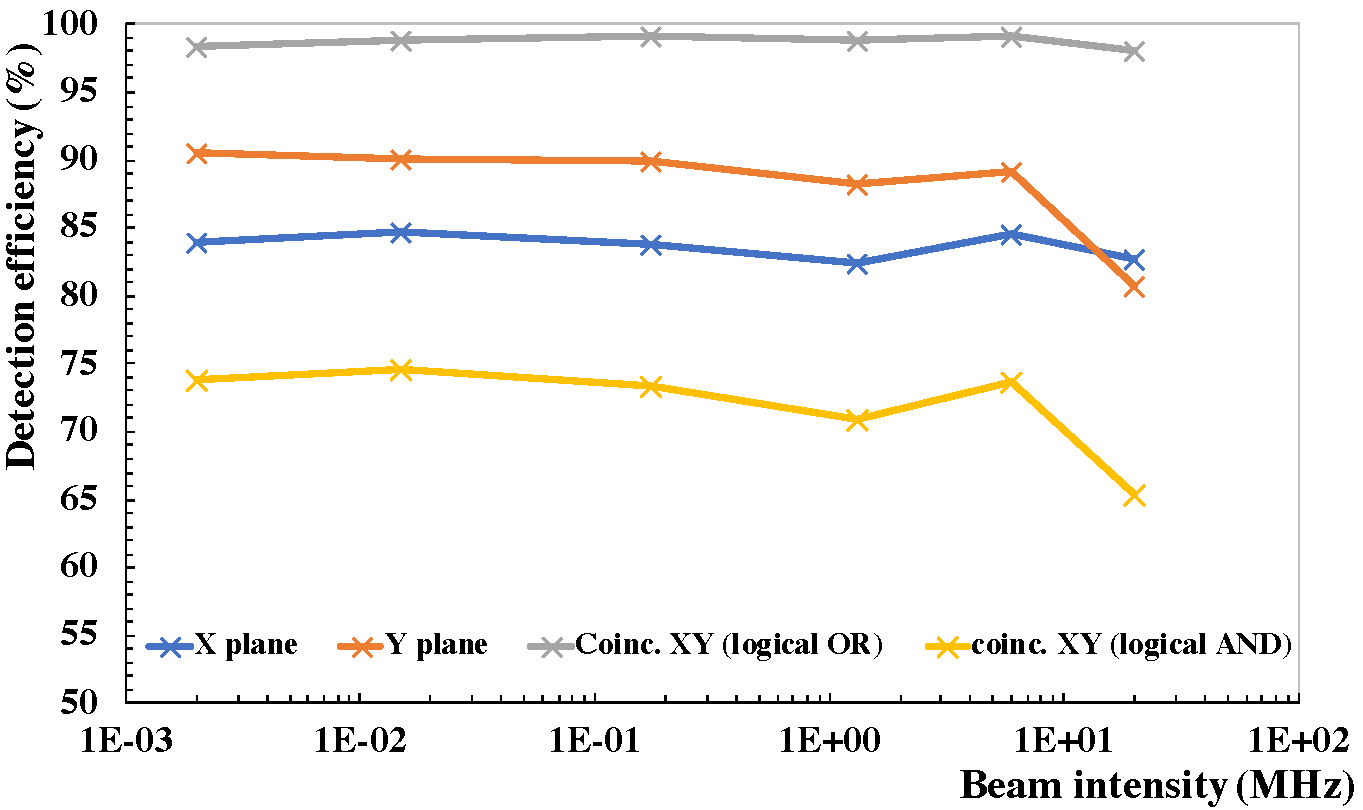
\includegraphics[width=0.7\textwidth]{figures/DE_March_2019_corr.pdf}
\caption{\small{\textit{Hodoscope  detection  efficiency  as  a  function  of  the proton beam intensity}}}
\label{fig:DE}
\end{figure}

\subsubsection{Time resolution}

The time resolution is evaluated by the difference between the trigger time given by the plastic scintillators placed upstream and downstream of the hodoscope and the recorded time of events involving at least one fiber in X and Y planes. The figure \ref{fig:Time_coinc} represents the distribution of these time differences for beam intensity of 43~kHz (\ref{fig:Time_43kHz}) and $\sim$10~MHz (\ref{fig:Time_10MHz}). The FWHM of the distributions are 0.5~ns and 2.5~ns respectively. A slight rising edge can be observed at 43~kHz and this increases when the beam intensity reach $\sim$10~MHz. Moreover, the distribution at $\sim$10~MHz reveals an additional regular signal particularly visible before and after the peak. About 5\% (resp.~20\%) of events are not in the range of the peak of time resolution for 43~kHz (resp.~$\sim$10~MHz).
\label{Time_resolution}

\begin{figure}[htb]
\centering
    \begin{subfigure}{0.49\textwidth} \centering 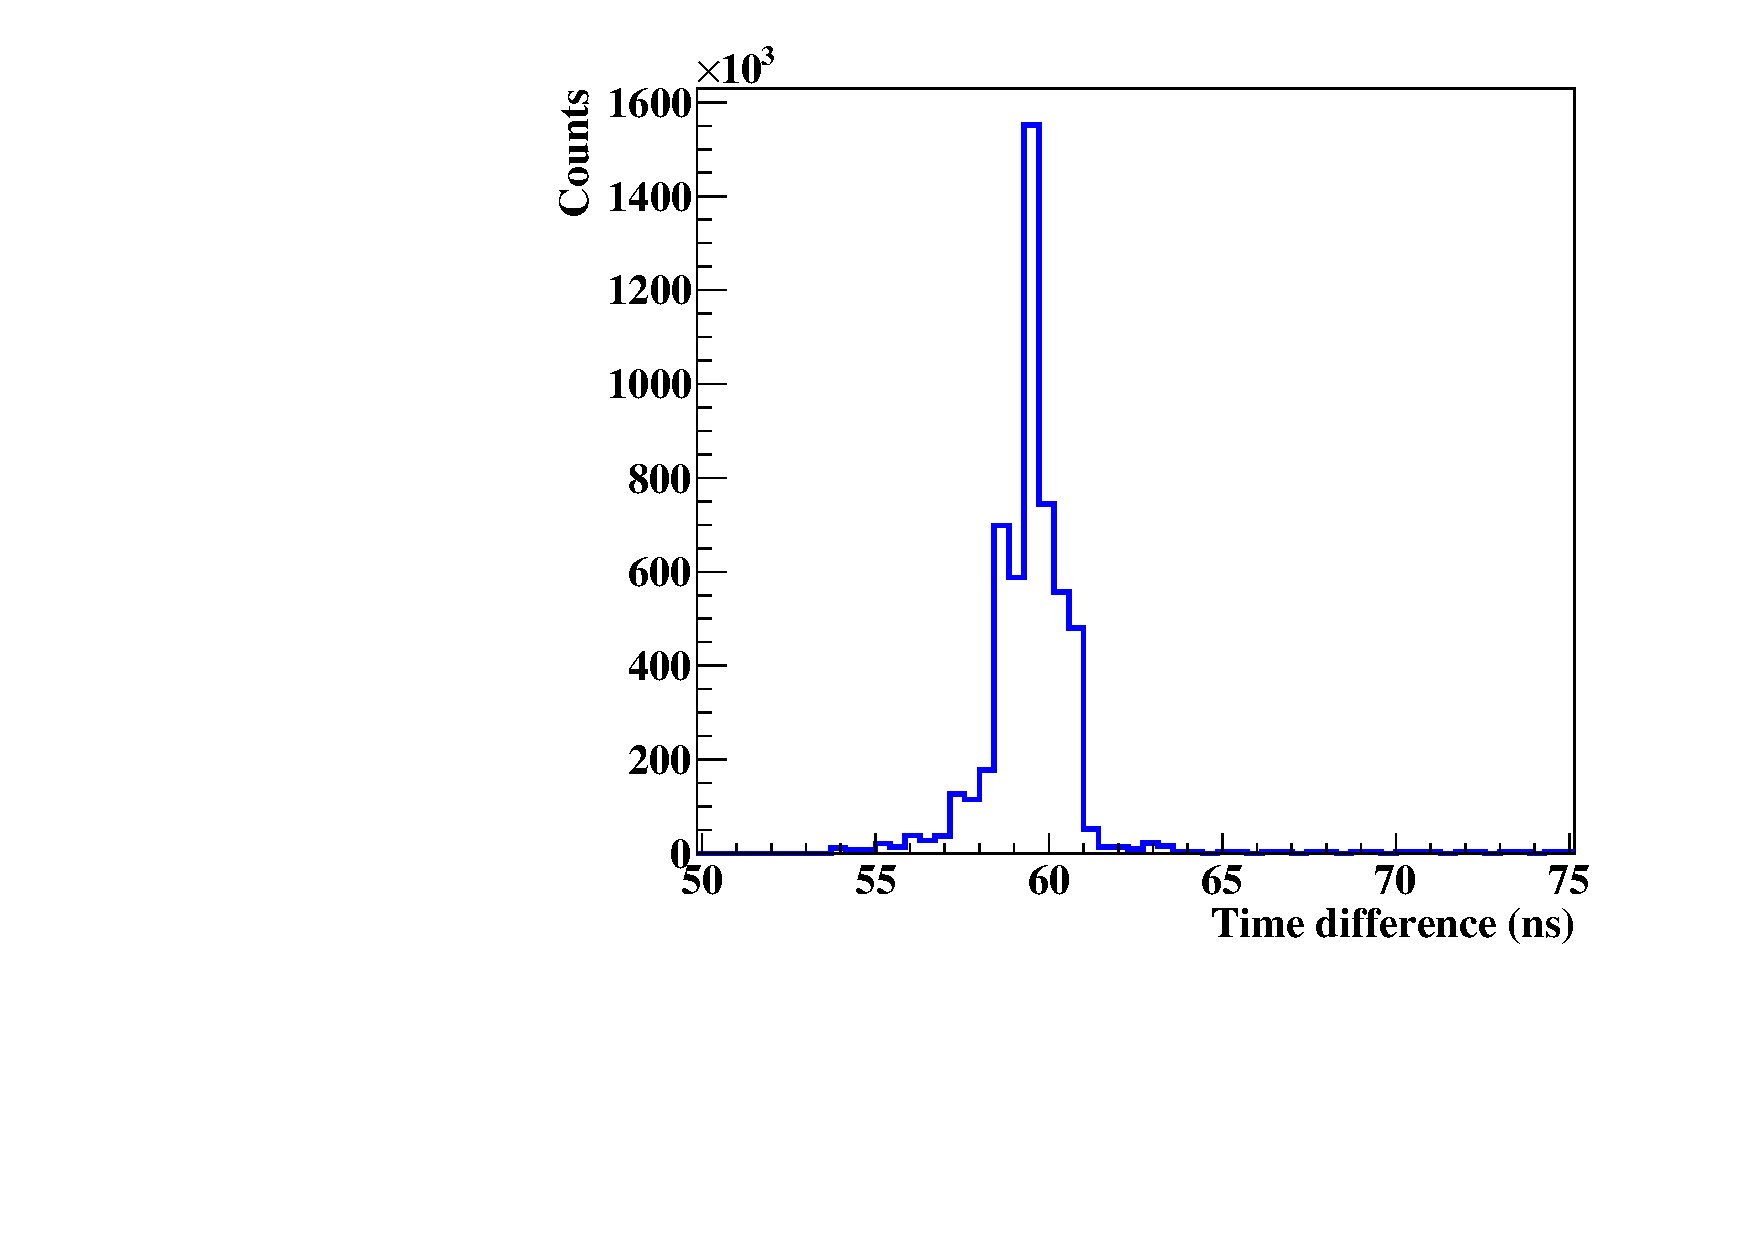
\includegraphics[width=\textwidth]{figures/time_coinc_43kHz_August.pdf} \caption{} \label{fig:Time_43kHz}
    \end{subfigure}
    ~
%\newline
%\centering
    \begin{subfigure}{0.49\textwidth} \centering 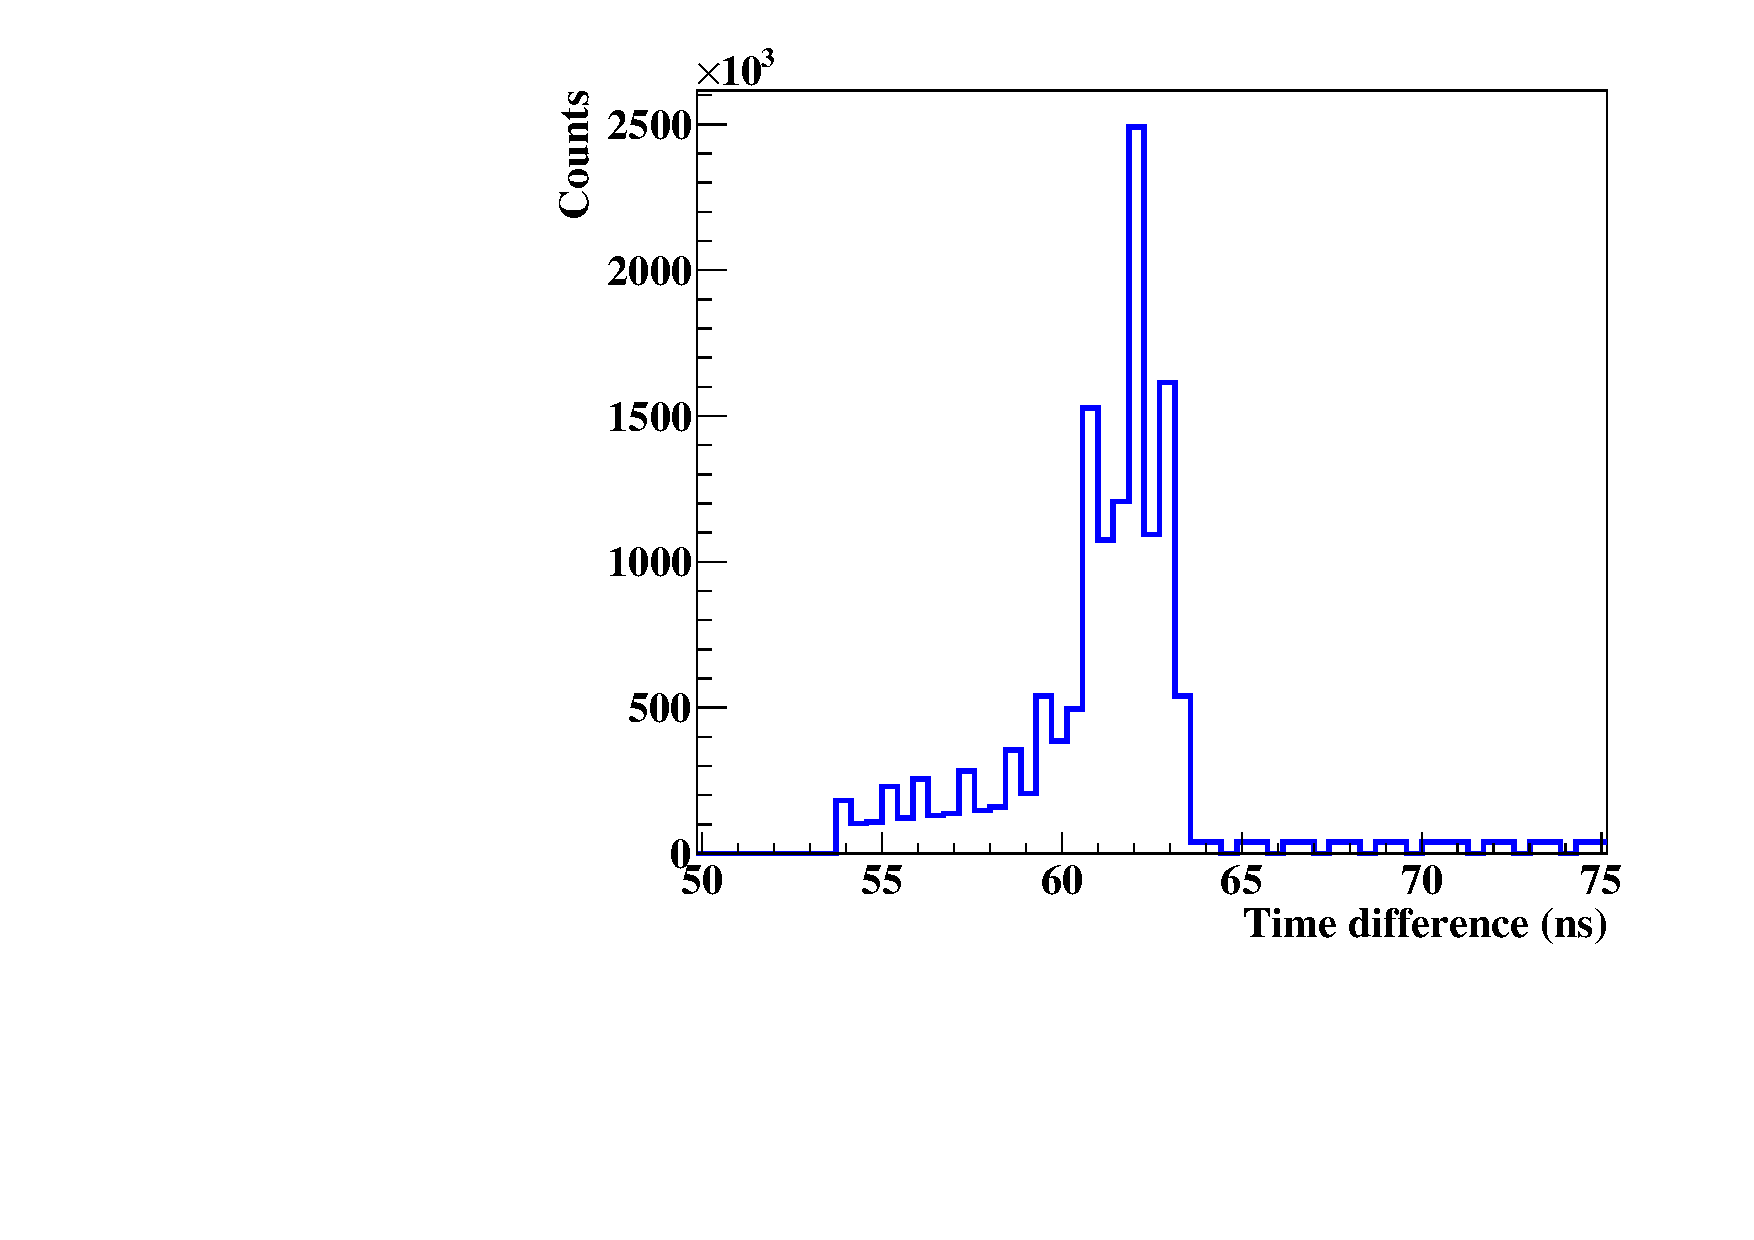
\includegraphics[width=\textwidth]{figures/time_coinc_10MHz_August.pdf} \caption{} \label{fig:Time_10MHz}
    \end{subfigure}
\caption{\small{\textit{Distribution of time difference between X and Y fibers and the trigger for beam intensity of 43~kHz (left) and $\sim$10~MHz (right).}}}
\label{fig:Time_coinc}
\end{figure}

\section{Discussion}

The experiment performed at GANIL represents the worst case for radiation damage in hadrontherapy (carbon ions with less than 3~cm range in water). During a single irradiation experiment, less than 10\% efficiency decrease was observed with (3.6$\pm$0.7)$\times$10$^{12}$~ions$\cdot$cm$^{-2}$, which represents more than 1000 clinical irradiations for the central hodoscope area, without accounting for the longer time scale recovery. Note that efficiency measurements performed at CAL-Nice used the same hodoscope, with a beam size largely overlapping the GANIL spot impact, years later.

Significant progress have been made in the development of firmware and configuration methods for acquisition boards. Thus, the beam tagging hodoscope is able to acquire data with a detection efficiency close to 75\% and a time resolution under 1~ns until $\sim$1~MHz intensities. However, these performances do not reach the specifications, namely, a detection efficiency of 90\% and a time resolution < 2~ns with a  beam intensity of $1\times 10^{8}$~MHz. Some physical phenomenons could explain the difference between the performances obtained and the expectations.

The assessment of the multiplicity highlighted a difference between the distributions in X and Y planes and the Poisson distribution, particularly for high beam intensities, which indicates that the multiplicity is not only due to statistical fluctuations. Electronic bounces in ASICs could be responsible for the rise of the multiplicity. Indeed, an electronic bounce of a previous event can be recorded in the time window of a new physical event, subsequently increasing the multiplicity rate. Moreover, bounces can generate additional triggers in a plane, which are not correlated to a signal to the other plane, inducing a decrease of the detection efficiency. The distribution of time difference between X and Y fibers and the trigger at $\sim$10~MHz (figure \ref{fig:Time_10MHz}) shows regular structures, reminiscent of electronic bounces.

The difference between M>1 rates in X and Y planes can be explained by the presence of a noisier ASIC to handle Y fibers plane than the one processing X fibers plane. The noisiest ASIC could be more sensitive to the accuracy of the setting method which was limited to threshold variation steps of 100 a.u and gain step of 0.25 during the current injection scans. It is worth of notice that the electronic circuit between the two ASICs and the FPGA is slightly different. The replacement of this ASIC and the modification of the electronic circuit could allow a reduction of the difference of response of the ASICs.

Although the time resolution of the CLaRyS hodoscope is lower than the other prototypes around the world, with a resolution over 2~ns at high intensity against less 1~ns, its performance is close to the expectation and an upgrade of the electronic components of the acquisition chain could allow to improve the time resolution. Otherwise, the detection efficiency assessed for a single plane (logical OR condition) is comparable to the other trackers. The detection efficiency with a logical AND between two planes with clinical intensities has not been currently reported in the other studies. Finally, the ability of the beam tagging hodoscope to be coupled to a beam monitoring device to provide trigger signals with 1~$\upmu$s delay as been recently demonstrated \cite{Chen2019}.


\section{Conclusion}

The different in-beam tests allowed to characterize the beam tagging hodoscope in terms of radiation damages, multiplicity, detection efficiency and time resolution. A methodology of configuration of the ASIC thresholds and input channel gains has been tested and allowed to obtain a detection efficiency higher than 98\% with a logical OR and 65\% with a logical AND between X and Y fiber planes. A time resolution <1~ns for intensities under 1~MHz was obtained with the new version of the acquisition firmware. A more accurate selection of ASIC thresholds and input channel gains selection during the current injection would slightly enhance the detection efficency of the beam tagging hodoscope. However, the modification of the ASIC chip and electronic circuit of the acquisition board is the main area for improvement of the beam tagging hodoscope performances under clinical intensities.

%\appendix
%\section{Example of appendix title}
%Please always give a title also for appendices.





\acknowledgments
This work was partially performed in the framework of Labex PRIMES (ANR-11-LABX-0063) and within the frame of the EU Horizon 2020 project RIA-ENSAR2/MediNet (654 002).  

%\paragraph{Note added.} This is also a good position for notes added after the paper has been written.



\bibliography{hodoscope_biblio}
\bibliographystyle{ieeetr}

% We suggest to always provide author, title and journal data:
% in short all the informations that clearly identify a document.

%\begin{thebibliography}{99}

%\bibitem{a}
%Author, \emph{Title}, \emph{J. Abbrev.} {\bf vol} (year) pg.

%\bibitem{b}
%Author, \emph{Title},
%arxiv:1234.5678.

%\bibitem{c}
%Author, \emph{Title},
%Publisher (year).


% Please avoid comments such as "For a review'', "For some examples",
% "and references therein" or move them in the text. In general,
% please leave only references in the bibliography and move all
% accessory text in footnotes.

% Also, please have only one work for each \bibitem.


%\end{thebibliography}
\end{document}
